\documentclass{VUMIFPSbakalaurinis}
\usepackage[table]{xcolor}
\usepackage{algorithmicx}
\usepackage{algorithm}
\usepackage{algpseudocode}
\usepackage{amsfonts}
\usepackage{amsmath}
\usepackage{bm}
\usepackage{caption}
\usepackage{color}
\usepackage{float}
\usepackage{graphicx}
\usepackage{listings}
\usepackage{subfig}
\usepackage{wrapfig}
\usepackage{tikz}

\usepackage{enumitem}
\setitemize{noitemsep,topsep=0pt,parsep=0pt,partopsep=0pt}
\setenumerate{noitemsep,topsep=0pt,parsep=0pt,partopsep=0pt}

% Ignore all trivial warnings
\hbadness=5000
% Titulinio aprašas
\university{Vilniaus universitetas}
\faculty{Informatikos institutas}
\department{Programų sistemų katedra}
\papertype{Bakalauro baigiamasis darbas }
\title{Rodiklių duomenų apdorojimo sistemų generavimas iš duomenų modelių}
\titleineng{Generation of Indicator Data Processing Systems\\from Data Models}
\author{Vytautas Žilinas}
\supervisor{lekt. Andrius Adamonis}
\reviewer{assoc. prof., dr. Karolis Petrauskas}
\date{Vilnius – \the\year}

% Nustatymai
% \setmainfont{Palemonas}   % Pakeisti teksto šriftą į Palemonas (turi būti įdiegtas sistemoje)
\bibliography{bibliografija}

\begin{document} 
\maketitle

\cleardoublepage\pagenumbering{arabic}
\setcounter{page}{2}

\sectionnonumnocontent{Santrauka}
Šį darbą sudaro teorinė ir eksperimentinė dalis. Teorinėje dalyje apibrėžiamas rodiklis, jo struktūra ir struktūros pokyčiai. Apibrėžiami kokie yra įmanomi pokyčiai ir kaip eksperimentinėje dalyje kuriamas sprendimas prie pokyčių prisitaikys. Specifikuojama duomenų struktūra ir duomenų struktūrų apjungimo ir skirtumo operacijas. Apibrėžiamas srautinis apdorojimas ir pasirenkama sistema, kuri bus naudojama eksperimentinėje dalyje. Remiantis gautais rezultatais
nustatoma, kad šiam uždaviniui spręsti pasirenkama "Heron" srautinio apdorojimo sistema. Remiantis pasirinkta srautinio apdorojimo sistema ir apibrėžta rodiklių duomenų struktūra, eksperimentui nusprendžiama generuoti srautinio apdorojimo modulius parašytus "Python" programavimo kalba. Eksperimentinėje dalyje remiantis pasiūlyta architektūra realizuojama bandomoji sistemos versija. Atliekant skirtingų kiekių rodiklių duomenų ir rodiklių duomenų pokyčių simuliaciją stebėjimais analizuojamas šios sistemos tinkamumas apibrėžtam uždaviniui spręsti. Gauti tyrimų rezultatai lyginami, pateikiamos išvados. Taip įrodoma, kad toks sprendimas gali būti įgyvendinamas ir kad kodo generavimas ir srautinio apdorojimo sistema "Heron" yra tinkamas sprendimas kintančių rodiklių uždaviniui spręsti.
\raktiniaizodziai{srautinis apdorojimas, kodo generavimas, rodiklis, rodiklio duomens pokyčiai}   

\sectionnonumnocontent{Summary}
This work consists of a theoretical and an experimental part. Theoretical part defines the indicator, its structure and changes in indicator structure. It define what changes are possible and how the developed solution in the experimental part will adapt to the changes, specifies the data structure and data structure merging and difference operations, defines stream processing and selects the system to be used in the experimental part. Based on the results it is determined that "Heron" stream processing system is chosen to solve this task. Based on the selected stream processing system and the defined data structure of indicator, it is decided to generate streaming modules written in "Python" programing language. In the experimental part, a pilot version of the system is implemented based on the proposed architecture. By doing the simulation using varying amounts of indicators and indicator changed, the suitability of this system for a defined task is tested. The results of this research are compared and conclusions are given. This demonstrates that such a solution can be implemented and that the code generation and streaming system "Heron" is the right solution to deal with the challenge of changing indicators.
\keywords{stream processing, code generation, indicator, indactor structure change}

\tableofcontents

\sectionnonum{Įvadas}
 
% TODO: Įžangoje apžvelgti srautinį apdorojimą ir kodo generavimą.
Šiame darbe yra nagrinėjamas rodiklių duomenų apdorojimas ir kuriamas koncepcinis sprendimas galintis prisitaikyti, kai keičiama rodiklių duomenų struktūrą. Rodiklių duomenimis vadinkime pasikartojančių įvykių parametrus aprašančius duomenis. Pavyzdžiui, įvairių matuoklių – temperatūros, resursų suvartojimo – fiksuojamus rodmenis, kasmėnesinius veiklos indikatorius, tokius kaip veiklos finansines ataskaitas ar veiklos procesų indikatorius. Taip pat rodiklių struktūra gali keistis laikui bėgant: objektų atributų taksonomija (pvz. mirties priežasčių sąrašas, finansinių sąskaitų sąrašas) arba įrašo atributų sąrašai. Surenkamu rodiklių duomenų kiekis visada didėja, taip pat ir duomenų kiekis, kuriuos reikia apdoroti pagal rodiklius auga, todėl standartiniai sprendimai, pavyzdžiui, reliacinės duomenų bazės netinka dėl ilgos apdorojimo trukmės. Rodiklių duomenų bazės pasižymi tuo, kad duomenys į jas patenka iš daug skirtingų tiekėjų ir patekimo laikas tarp tiekėjų nėra sinchronizuojamas, o suagreguotą informaciją vartotojai gali užklausti bet kurio metu. Todėl šiame darbe bus nagrinėjamas srautinis duomenų apdorojimas, kuris patenkančius duomenis apdoros realiu laiku, ir saugos jau apdorotus. \par
Realaus laiko duomenų apdorojimas (angl. Real-time data processing) yra jau senai nagrinėjamas, kaip vienas iš būdų apdoroti didelių kiekių duomenis (angl. Big data). Vienas iš realaus laiko apdorojimo sprendimų yra srautinis duomenų apdorojimas. Srautinis duomenų apdorojimas (angl. stream processing) – lygiagrečių programų kūrimo modelis, pasireiškiantis sintaksiškai sujungiant nuoseklius skaičiavimo komponentus srautais, kad kiekvienas komponentas galėtų skaičiuoti savarankiškai \cite{shortstreamproc}. Darbe yra analizuojamos jau egzistuojančias srautinio apdorojimo sistemų programas pagal srautinio apdorojimo programų savybes aprašytas Michael Stonebraker, pasirenkama vieną srautinio apdorojimo programa ir pagal ją sukuriamas koncepcinis sprendimas. 
\par
Kadangi rodikliai laikui bėgant gali būti keičiami reikia, kad sprendimas, galėtų prisitaikyti prie pokyčių. Yra keli būdai kaip tai tokie sprendimai gali būti kuriami:
\begin{itemize}
    \item Rankinio atnaujinimo sprendimas. Sukuriamas sprendimas pagal esamus reikalavimus, o atsiradus naujiems reikalavimams būtų kuriamos naujos arba keičiamos esamas apdorojimo sistemos. 
    \item Universalus sprendimas. Sukuriamas universalus parametrizuojamas sprendimas ir pritaikomas užduotims nustatant parametrus.
    \item Kodo generavimo sprendimas. Sukuriamas sprendimas, kuris generuoja srautinio duomenų apdorojimo sistemas pagal iš anksto aprašytą struktūrą.  
\end{itemize}   
Tinkamas sprendimas turi būti išrinktas pagal sprendžiamą problemą. Jei nėra numatomas kitimas, pagal ką turi būti apdorojami duomenys, tai galima pasirinkti ir rankinio apdorojimo sprendimą, kadangi nėra didelės tikimybės, kad teks keisti sprendimą. Toks sprendimas tiktų apdorojant išmaniųjų skaitiklių duomenis \cite{skaitikliai}. Universalus sprendimas taip pat gali būti tinkamas jei įeinantis duomenis yra specifiški ir yra poreikis juos visus apdoroti. Toks sprendimas gali būti aktualus apdorojant duomenis iš sensorių, kurie matuoja namų būsena (temperatūra, drėgmę ir t.t.) ir bet koks naujas sensorius taip pat turi būti prijungtas ir apdorotas \cite{yang2017iot}. Šiame darbe buvo norima nagrinėti kodo generavimo sprendimo tinkamumą užduotims. \par
Pagal Jack Herrington 2003 metų knygą "Code Generation in Action" kodo generavimas - tai rašymas programinės įrangos, kuri rašys reikiamą programinę įrangą problemai spręsti. Tai daroma tokiais atvejais, kai sprendžiama problema reikalauja daug rankinio darbo, kurį įmanoma automatizuoti. Kuo didesnio sprendimo reikalauja uždavinys tuo patraukliau tampa naudoti kodo generavimą sprendimo kūrimui. Kodo generavimas suteikia tokius privalumus: 
\begin{itemize}
    \item Architektūrinį nuoseklumą: 
    \begin{itemize}
        \item Verčia programuotojus labiau mąstyti apie architektūrą.
        \item Jei sunku "priversti" generatorių generuoti reikiamą kodą, problema gali būti architektūroje.
        \item Geros dokumentacijos buvimas sumažina problemą, kai nariai palieką projektą.
    \end{itemize}
    \item Abstrakciją:
    \begin{itemize}
        \item Programuotojai galės kurti naujus šablonus, kurie leis esamą funkcionalumą pritaikyti kitomis kalbomis, sprendimais daug paprasčiau negu rankomis parašytą kodą.
        \item Verslo analitikai gali apžvelgti ir patvirtinti sprendimo abstrakciją.
        \item Abstrakcija padės paprasčiau paruošti dokumentacija, testavimo atvejus, produkto palaikymo medžiagą ir t.t.  
    \end{itemize}
    \item Aukštą komandos moralę - rašomas kodas bus nuoseklus ir kokybiškas todėl kels komandos pasitikėjimą.
    \item Tinkamas sprendimas Judriajam programavimui, kadangi kodo generavimo kuriami sprendimai yra lankstesni, tai leidžia ateityje juos lengviau keisti ir atnaujinti.   
\end{itemize} 
Kodo generavimas tampa tikrai naudingas tada, kai jis naudojamas didelių kiekių rankiniam kodavimui pakeisti \cite{herrington2003code}. \par
Darbe nagrinėjamas architektūra ir koncepcinis sprendimas generuojantis srautinio apdorojimo sistemas pagal rodiklių duomenų modelius. Rodiklių duomenis apdorojantis koncepcinis sprendimas turi pasižymėti tokiomis savybėmis: 
\begin{itemize}
    \item Galėjimas keisti esamas apdorojimo sistemas, kai pakeičiamas rodiklių duomenų modelis.
    \item Išvestinių rodiklių gavimas iš daugiau nei vieno rodiklio transformacijos.
    \item Išvestinių rodiklių apdorojimas pagal iš anksto apibrėžtas funkcijas.
    \item Srautinių apdorojimo sistemų generavimas pagal deklaratyvų aprašymą.
\end{itemize}  

Tikslas: Sukurti rodiklių duomenų srautinio apdorojimo sistemos, pritaikomos prie duomenų struktūrų naudojant kodo generavimą, architektūrą.

Uždaviniai:
\begin{enumerate}
    \item Apibrėžti rodiklių duomenų modelį ir galimus rodiklių duomenų struktūros pokyčius.
    \item Atlikus šaltinių analizę pasirinkti srautinio duomenų apdorojimo programinę įrangą.
    \item Sudaryti srautinio apdorojimo sistemos architektūrą, pagal ją sukurti koncepcinį sprendimą. 
    \item Nustatyti sukurto koncepcinio sprendimo ir architektūros savybes atliekant bandymus su rodiklių duomenimis.
\end{enumerate}

\section{Rodiklių duomenys}

Rodiklių duomenimis vadinkime pasikartojančių įvykių parametrus aprašančius duomenis. Rodiklių duomenys pasižymi tuo, jog yra aktualus, kai jie jau yra apdoroti. Taip pat rodikliai yra nepastovūs, jų struktūra gali būti keičiama - atsirasti naujų savybių, kurias reikia surinkti arba yra pašalinamos jau esamos savybės. Rodiklių duomenys yra renkami ir analizuojami labai skirtingiems poreikiams - visur kur reikalinga statistika ir apdorojami didelį kiekiai duomenų yra naudojami rodikliai: tai gali būti įmonės vedamą "Microsoft Excel" skaičiuoklė, kurioje užrašyta kiek buvo mokėta už elektrą kiekvienais metais per paskutinius 10 metų arba juodosios skylės nuotrauka padaryta koreliuojant didelio duomenų kiekį iš 8 skirtingų teleskopu ir gauti rodikliai rodo taškus ant paveikslėlio, kurio dydis yra \(10^{12}\) kartų mažesnis nei pradiniai duomenys \cite{akiyama2019first}. \par    
Pirmiausiai turime apibrėžti bendrą rodiklių duomenų modelį, kurio pagalba galėtume apibrėžti rodiklius. 

\subsection{Pirminiai rodiklių duomenys}

Rodiklių duomenys yra gaunami apdorojus pirminius rodiklių duomenis, kurie susidaro iš raktų ir reikšmių žodyno (\ref{img:duomenys} pav.), kur raktas gali būti tik tekstinio tipo, o reikšmė - tekstas arba skaičius. Duomenų raktai ir raktų kiekis gali nesutapti, vieni žodynai gali turėti daugiau raktų-reikšmių elementų, kitų raktai gali būti visiškai nesusiję su apdorojamais rodikliais. \par 
Kadangi pirminiai rodiklių duomenys gali būti gaunami iš skirtingų šaltinių, skirtingais laikais, todėl kuriamas sprendimas turi galėti priimti duomenis asinchroniškai ir iš skirtingų šaltinių, o sprendimas realiu laiku turi sugebėti apdoroti reikiamus duomenis, o nereikalingus atmesti. 

\begin{figure}[H]
    \centering
    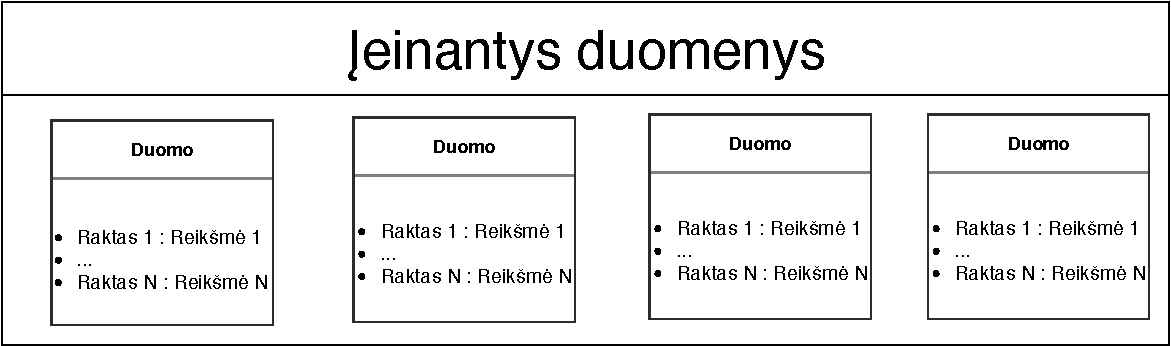
\includegraphics[width=1\textwidth]{img/duomenys.pdf}
    \caption{Įeinantys duomenys}
    \label{img:duomenys}
\end{figure}

\subsection{Rodiklių duomenų modelis}

Norit apdoroti daug skirtingų rodiklių turime apsibrėžti bendrą rodiklių duomenų modelį (\ref{img:rodiklio_apibrezimas} pav.), pagal kurį bus generuojamos srautinio duomenų apdorojimo sistemos. Siūlomas apibrėžimas susidaro iš trijų dalių: 
\begin{itemize}
    \item Rodiklių duomenų pirminis raktas sudarytas iš įeinančių duomenų raktų rinkinio.
    \item Įeinančių duomenų reikšmių srities apribojimai.
    \item Įeinančių duomenų raktų rinkinys, kuris aprašo rodiklius ir išvestinių rodiklių kombinavimo apibrėžimai. 
\end{itemize}

\begin{figure}[H]
    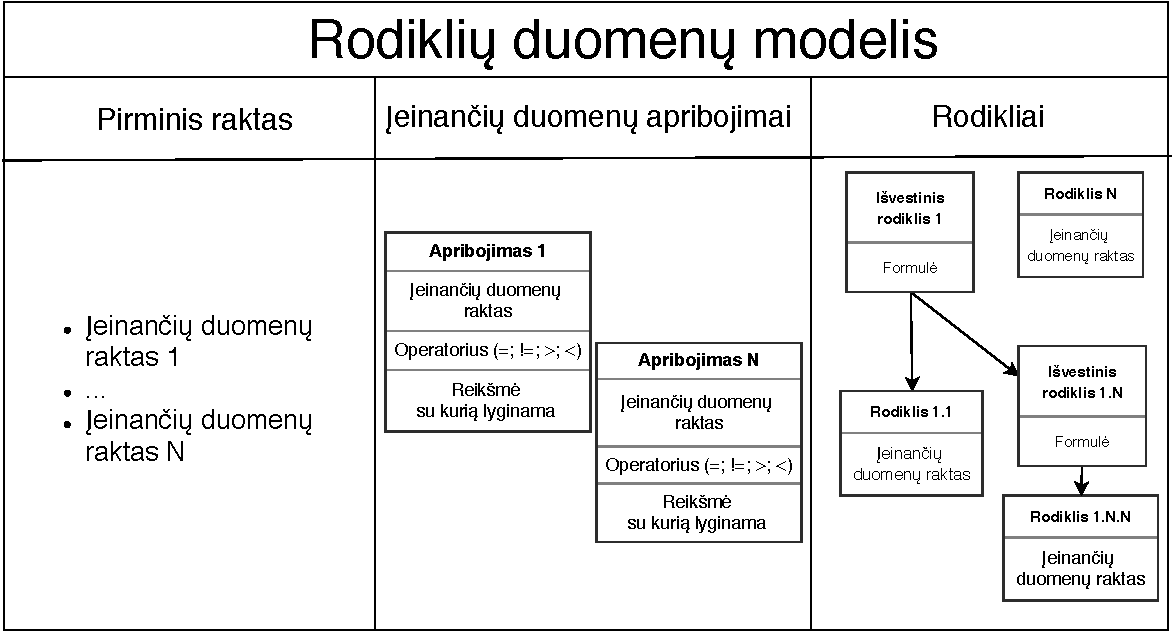
\includegraphics[width=1\textwidth]{img/rodiklio_modelis.pdf}
    \caption{Rodiklių duomenų modelis}
    \label{img:rodiklio_apibrezimas}
\end{figure}

\subsubsection{Pirminis raktas}

Pirma rodiklio apdorojimo apibrėžimo dalis nusako raktų rinkinį reikšmių pagal kurias grupuojami apdoroti duomenis. Pavyzdžiui:
\begin{itemize}
    \item Statistikos srityje: norint surinkti duomenis aprašančius \textbf{skirtingų savivaldybių} nekilnojamo turto kainas pagal \textbf{metus}, raktų rinkinys atrodys taip: \[\{\textit{"Savivaldybė", "Metai"}\}\]
    \item Sensoriniai rodikliai: norint surinkti vienos dienos duomenis aprašančius \textbf{skirtingų sensorių} parodymus \textbf{kiekvieną valandą}, \textbf{kiekvienam ofiso kabinetui}, raktu rinkinys atrodys taip: \[\{\textit{"Sensoriaus tipas", "Valanda", Kabineto Numeris}\}\] 
    \item Buhalterijoje: norint surinkti duomenis parodančių kiek ir \textbf{kokie skyriai} patyrė išlaidų kiekvieną šių \textbf{metų mėnesį}, raktų rinkinys atrodys taip: \[\{\textit{"Skyriaus pavadinimas", "Mėnesis"}\}\] 
\end{itemize}  \par
Raktų kiekis neturi būti ribojamas, kadangi realiame pasaulyje yra neribotas kiekis duomenų pagal kuriuos galima grupuoti. Visų raktų reikšmių kiekių sandauga - apdorotų rodiklių duomenų pirminių raktų aibė. 

\subsubsection{Įeinančių duomenų apribojimai}

Antra rodiklio duomenų modelio dalis susidaro iš masyvo apribojimų, kurie aprašo kokie duomenys turi būti apdorojami, o kokie ne. Apribojimas yra aprašomi kaip predikatai.
Pavyzdžiui:
\begin{itemize}
    \item Statistikos srityje: norint surinkti žmonių, \textbf{vyresnių nei 60 metų} atlyginimus pagal kalendorinius metus, apribojimų sąrašas atrodys taip: \[\textit{"Amžius" > 59}\]
    \item Sensoriniai rodikliai: norint surinkti \textbf{tik savaitgalio} sensorių rodiklius, apribojimų sąrašas atrodys taip: \[\textit{"Savaitės Diena" > 5}, \textit{"Savaitės Diena" < 8}\]
    \item Buhalterijoje: norint apdoroti tam tikrus duomenis \textbf{tik "Marketingas" skyriaus} apribojimų sąrašas atrodys taip: \[\textit{"Skyriaus pavadinimas" == "Marketingas"}\] 
\end{itemize}  
Apribojimų kiekis yra neribojamas. Šie apribojimai turi leisti naudoti tuos pačius duomenis skirtingiems rodikliams ir rodiklių rinkiniams apdoroti. Įeinantis duomenys turi būti ribojami pagal reikšmes, kurios turi priklausyti apribojimų aibių sankirtai. Jei yra pateikti du apribojimus, tai įeinančio duomens ribojamos reikšmės turi patekti į abiejų apribojimų aibes. 
\par

\subsubsection{Rodikliai}
Rodiklių duomenų modelio dalis, kuri aprašo, kokie rodikliai renkami iš pradinių duomenų ir išvestinių rodiklių formules. 
Ši dalis susidaro iš masyvo medžių. duomenis medžio šakomis eina iš apačios į viršų. Kiekviena medžio viršūnė saugo apdorotą rodiklį ir talpiną jį duomenų bazėje. Medžio viršūnės gali aprašyti du skirtingus dalykus: rodiklį ir išvestinį rodiklį. \par
Rodiklis gauna ir apdoroja įeinančius duomenis. Rodiklio apibrėžimas susidaro iš įeinančių duomenų elemento rakto, reikšmės kuri bus naudojama apdorojimui. Rodikliuose ši reikšmė visada yra skaitinė, ji gali nurodyti skaičiuojamas savybes arba tai gali būti dvejetainė reikšmė. \par
Išvestinis rodiklis gauna duomenis iš prieš tai ėjusio rodiklio. Išvestinio rodiklio gaunami duomenys - tai prieš tai ėjusios viršūnės bet kokio rodiklio paskutinė reikšmė. Kaip duomenis bus apdoroti išvestinio rodiklio viršūnėje aprašo formulė, kurioje pateikiama veiksmai atliekami su prieš tai ėjusių viršūnių paskutinėmis reikšmėmis ir atliekami susiejant duomenis unikaliu identifikatoriumi, kuris sukuriamas kiekvienam įeinančiam duomeniui patenkant į apdorojimo sprendimą. Norint rodiklį gauti ne tik naudojant pagrindinius matematinius veiksmus kaip sudėtis arba atimtis, turi būti įmanoma naudoti, bet kokį iš anksto aprašytą metodą duomenims apdoroti. \par
Pavyzdžiui:
\begin{itemize}
    \item Statistikos srityje: norint surinkti rodiklių duomenis nekilnojamo turto kainų ir žmonių kaitos šalyje (\(\textit{Žmonių kaita} = (\textit{Gimstamumas - Mirtingumas}) + (\textit{Migracija} * \textit{Gyventojų kiekis}\)), renkamų rodiklių medžiai apsirašytų taip: 
    \[	
        
\begin{tikzpicture}[sibling distance=7em, every node/.style = {shape=rectangle, rounded                                corners, draw, align=center,	
            top color=white, bottom color=white}]	
            \node{Nekilnojamo turto kaina};
        \end{tikzpicture} 
    \]
    \[
        \begin{tikzpicture}[sibling distance=10em,
            level distance=2cm,
            every node/.style = {shape=rectangle, rounded corners,	
                                 draw, align=center,	
                                 top color=white, bottom color=white}]	
            \node{Žmonių kaita\\Nuolatinė kaita + (Migracija * Gyventojų kiekis)}
                    child { node {Nuolatinė kaita\\Gimstamumas - Mirtingumas} 
                            child {node {Mirtingumas}}
                            child {node {Gimstamumas}} }	
                    child { node {Migracija} } 	
                    child { node {Gyventojų kiekis} }; 	
        \end{tikzpicture} 	
    \]
    \item Sensoriniai rodikliai: norint surinkti drėgmės, temperatūros ir šviesos sensorių rodiklius, rodiklių medžiai atrodys taip:
    \[	
        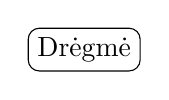
\begin{tikzpicture}[sibling distance=7em,  every node/.style = {shape=rectangle,  
                                rounded corners, draw, align=center,	
                                top color=white, bottom color=white}]	
            \node{Drėgmė};
        \end{tikzpicture}\>\>\>\>
        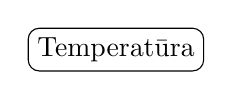
\begin{tikzpicture}[sibling distance=7em, every node/.style = {shape=rectangle, 
                                rounded corners, draw, align=center,	
                                top color=white, bottom color=white}]	
            \node{Temperatūra};
        \end{tikzpicture}\>\>\>\>
        
\begin{tikzpicture}[sibling distance=7em, every node/.style = {shape=rectangle, rounded                                corners, draw, align=center,	
                                top color=white, bottom color=white}]	
            \node{Šviesa};
        \end{tikzpicture} 	
    \]
    \item Buhalterijoje: norint suskaičiuoti kiek įmonės darbuotojai gauna pajamų (\(\textit{Pajamos} = (\textit{Atlyginimas}/1.7) + \textit{Premijos}\)) rodiklių medis bus toks: 
    \[	
        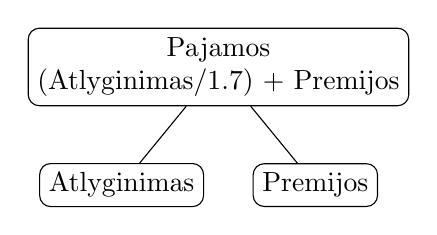
\begin{tikzpicture}[sibling distance=7em,	
            every node/.style = {shape=rectangle, rounded corners,	
                                 draw, align=center,	
                                 top color=white, bottom color=white}]	
            \node {Pajamos\\(Atlyginimas/1.7) + Premijos}	
                    child { node {Atlyginimas} }	
                    child { node {Premijos} } ;	
        \end{tikzpicture} 	
    \]
\end{itemize}  


\subsection{Rezultatų struktūra}

Apdorotų rodiklių rezultatai gauti iš pirminių rodiklių duomenų sudaro lentelę. Lentelės duomenų pirminis raktas yra sudarytas iš pirminių rodiklių duomenų reikšmių kombinacijos gautos pagal rodiklio modelio pirminį raktą. Rezultatų lentelės stulpeliai susidaro iš priminio rakto ir išvestinių rodiklių. Rezultatų lentelės išvestinių rodiklių kolonėlės susidaro iš apdorotų rodiklių duomenų.

\begin{figure}[H]
    \centering
    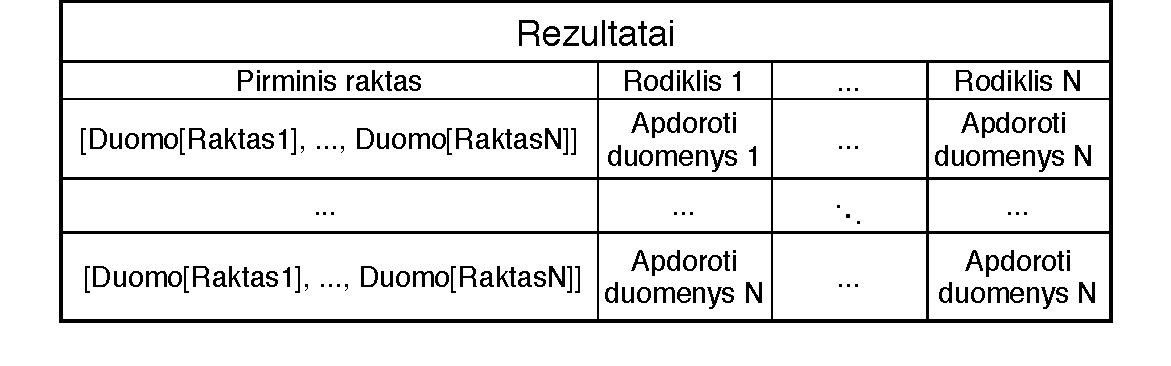
\includegraphics[width=1\textwidth]{img/rezultatai.pdf}
    \caption{Rezultatų struktūra}
    \label{img:rezultatai}
\end{figure}

\subsection{Rodiklių duomenų struktūros kitimas}

Rodiklių duomenų struktūra gali būti keičiama laikui bėgant. Buhalterijos srityje tai gali būti dėl naujo įstatymo, kuris pakeičia kažkurių rodiklių skaičiavimo formulę. Tai gali būti naujos rūšies išmaniųjų namų sensorius, kuriuo duomenys norima irgi rinkti, kad galėtume matyti pilną vaizdą. Statistikos srityje gali atsirasti poreikis išskaidyti tam tikrus rodiklius į mažesnes dalis, pavyzdžiui rinkti ne migracijos rodiklį kaip vieną, o atskirai emigraciją ir imigraciją. \par
Pagal mūsų aprašyta rodiklių duomenų modelį, mes taip pat turime apsibrėžti kas gali keistis:
\begin{itemize}
    \item Pirminis raktas negali keistis, nes naujos reikšmės tampa nepalyginamos su anksčiau surinktomis. Tarkim buvo renkami rodikliai metinių duomenų, o pagal poreikius reikia rinkti mėnesinius duomenis, ir lyginimas su anksčiau surinktais tampa neįmanomas. Todėl bet kokius pirminio raktus pokyčius turime laikyti nauju rodikliu. 
    \item Apribojimai gali keistis, tačiau šie pokyčiai turi turėti prasmę ir naudojami tik tam, kad būtų išlaikytos tos pačios apdorojamu įeinančių duomenų aibės. Tarkime mums reikėjo apdoroti duomenis iš visų skyrių išskyrus administraciją ir tokiam uždaviniui buvo sukurtas apribojimas - \(\textit{"Skyriaus pavadinimas" != "Administracija"}\). Tačiau po laiko dalis administracijos skyriaus atsiskyrė ir susikūrė naujas HR skyrius. Norint, kad būtų išlaikyta apdorotų rodiklių lyginimo prasmė, nauji apribojimai atrodys taip: \(\textit{"Skyriaus pavadinimas"!="Administracija"}, \textit{"Skyriaus pavadinimas"!="HR"}\)
    \item Rodikliai ir išvestiniai rodikliai gali būti keičiami: rodiklių medžio viršūnės gali būti pridedamos ir pašalinamos. Operacijos su rodikliais neturi įtakoti kitų rodiklių būsenos ir modelį. Tarkime jog skaičiavome pajamas naudodami formulę: \[\textit{Pajamos = Atlyginimas + Premijos}\] Ir pagal šią formulę buvo sukurtas toks rodiklių medis: 
    \[	
        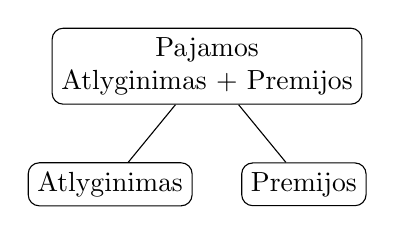
\begin{tikzpicture}[sibling distance=7em,	
            every node/.style = {shape=rectangle, rounded corners,	
                                 draw, align=center,	
                                 top color=white, bottom color=white}]	
            \node {Pajamos\\Atlyginimas + Premijos}	
                    child { node {Atlyginimas} }	
                    child { node {Premijos} } ;	
        \end{tikzpicture} 	
    \]\par
     Po tam tikro laiko atsirado poreikis pajamas skaičiuoti pagal formulę: \[\textit{Pajamos = Atlyginimas + Premijos + Komandiruočių dienpinigiai}\] Pagal naują formulę rodiklių medis turės atrodyti taip: 
     \[	
        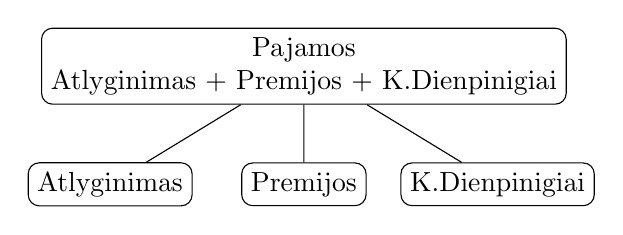
\begin{tikzpicture}[sibling distance=7em,	
            every node/.style = {shape=rectangle, rounded corners,	
                                 draw, align=center,	
                                 top color=white, bottom color=white}]	
            \node {Pajamos\\Atlyginimas + Premijos + K.Dienpinigiai}	
                    child { node {Atlyginimas} }	
                    child { node {Premijos} } 
                    child { node {K.Dienpinigiai} };	
        \end{tikzpicture} 	
    \]
\end{itemize} 

\noindent 
\section{Srautinio duomenų apdorojimo sprendimų analizė}

\subsection{Srautinis duomenų apdorojimas} \label{strprocess}

Siekiant apžvelgti modernius srautinio duomenų apdorojimo sprendimus turime apsibrėžti jų savybes.
2005 metais Michael Stonebraker apibrėžė 8 taisykles realaus laiko (angl. real-time) srautinio duomenų apdorojimo architektūrai \cite{stonebraker20058}:
\begin{enumerate}[label=\arabic*]
    \item taisyklė: Duomenys turi judėti. Žemo uždelstumo užtikrinimui sistema turi apdoroti duomenis nenaudojant duomenų saugojimo operacijų. 
    Taip pat sistema turi ne pati užklausti duomenų, o gauti juos iš kito šaltinio asinchroniškai. 
    \item taisyklė: Duomenų transformacijos turi būti vykdomas SQL pobūdžio užklausomis. Žemo abstrakcijos lygmens srautinio apdorojimo sistemos reikalauja ilgesnio programavimo laiko ir brangesnio palaikymo. Tuo tarpu aukšto abstrakcijos lygmens sistema naudojanti SQL užklausas, kurias žino dauguma programuotojų ir yra naudojamos daugelyje skirtingų sistemų, leidžia efektyviau kurti srautinio apdorojimo sprendimus.
    \item taisyklė: Architektūra turi susidoroti su duomenų netobulumais. Architektūra turi palaikyti galimybę nutraukti individualius skaičiavimus tam, kad neatsirastų blokuojančių operacijų, kurios sustabdo vieno modulio veikimą ir tuo pačiu visos architektūros veikimą. Taip pat ši architektūra turi sugebėti susidoroti su vėluojančiomis žinutėmis, pratęsiant laiko tarpą, per kurį ta žinutė turi ateiti.
    \item taisyklė: Architektūra turi būti deterministinė. Kiekvieną kartą apdorojant tuos pačius duomenis rezultatai turi būti gaunami tokie patys.
    \item taisyklė: Architektūra turi gebėti apdoroti išsaugotus duomenis ir realiu laiku gaunamus duomenis. Sistema parašyta su tokia architektūra turi galėti apdoroti jau esančius duomenis taip pat kaip ir naujai ateinančius. Toks reikalavimas buvo aprašytas, nes atsirado poreikis nepastebimai perjungti apdorojimą iš istorinių duomenų į realiu laiku ateinančius duomenis automatiškai.
    \item taisyklė: Architektūra turi užtikrinti duomenų saugumą ir apdorojimo prieinamumą. Kadangi sistema turi apdoroti didelius kiekius duomenų, architektūra klaidos atveju, turi sugebėti persijungti į atsarginę sistemą ir tęsti darbą toliau. Taip pat tokios klaidos atveju atsarginė sistema turi būti apdorojusi visus duomenis ir sugebėti iš karto priimti naujus duomenis, o ne apdoroti duomenis iš pradžių.
    \item taisyklė: Architektūra turi užtikrinti sugebėjimą paskirstyti sistemos darbus automatiškai. Srautinio apdorojimo sistemos turi palaikyti kelių procesoriaus gijų operacijas. Taip pat sistema turi galėti veikti ant kelių kompiuterių vienu metu ir prireikus paskirstyti resursus pagal galimybes.
    \item taisyklė: Architektūra turi apdoroti ir atsakyti akimirksniu. Anksčiau minėtos taisyklės nėra svarbios, jeigu sistema nesugeba greitai susidoroti su dideliu kiekiu naujų duomenų. Todėl turi būti naudojamas ne tik teisingas ir greitas srautinio apdorojimo sprendimas, bet ir gerai optimizuota sistema.
\end{enumerate}\par 
Todėl norint sužinoti tam tikro srautinio duomenų apdorojimo sprendimo tinkamumą uždaviniui reikia išanalizuoti jų savybes.   
\subsection{Srautinio duomenų apdorojimo sistemos}

Norime nustatyti srautinio apdorojimo sistemų savybes pagal:
\begin{itemize}
    \item Pristatymo semantika (angl. delivery semantics) - apibrėžia pagal kokį modelį bus pristatyti duomenys. Egzistuoja trys semantikos \cite{ensar20}: 
    \begin{itemize}
        \item Bent vieną kartą (angl. at-least-once) užtikrina, kad duomenys bus apdoroti bent kartą, bet gali atsirasti dublikatų. 
        \item Ne daugiau vieno karto (angl. at-most-once) užtikrina, kad duomenys bus apdoroti daugiausiai tik vieną kartą, bet gali atsirasti praradimų. 
        \item Tiksliai vieną kartą (angl. exactly-once) užtikrina, kad duomenys bus apdoroti tik vieną kartą ir klaidos bus suvaldytos.
    \end{itemize}
    \item Uždelstumas (angl. latency) - apibrėžia laikų sumą - kiek laiko trūko viena operacija ir kiek laiko ši operacija turėjo laukti eilėje kol bus pabaigtos kitos operacijos \cite{karimov2018benchmarking}.
    \item Pralaidumas (angl. throughput) - apibrėžia kiek pavyks įvykdyti operacijų per tam tikrą laiko tarpą.
    \item Abstrakcijos lygmuo (angl. abstraction) - apibrėžia kokio lygmens programavimo sąsają pateikia sprendimas.
\end{itemize}
Tam išnagrinėsime ir palyginsime, kaip šitas savybes išpildo keturi egzistuojantys srautinio apdorojimo sprendimai - "Apache Storm", "Apache Spark", "Apache Flink" ir "Heron".
% \begin{table}[!htbp]
%     \begin{center}
%         \caption{Srautinių duomenų apdorojimo sprendimų palyginimas}
%         \label{table:comparer}
%         \begin{tabular}{ | l | p{12cm} |}
%             \hline
%             \cellcolor[gray]{0.8} Charakteristika &  Išpildymas \\* \hline
%             \cellcolor[gray]{0.9} Pristatymas & "Apache Spark" ir "Apache Flink" sprendimų pristatymo semantika yra tiksliai vieną kartą (angl. exactly-once), tai reiškia, kad visi duomenys bus apdoroti tik vieną kartą. Tačiau tam, kad užtikrinti šią semantiką sprendimas sunaudoja daug resursų, kadangi reikia užtikrinti, kad operacija bus vykdoma būtent vieną kartą kiekviename srautinio apdorojimo žingsnyje: duomenų gavime, kuris stipriai priklauso nuo duomenų šaltinio, duomenų transformacijos, kurią turi įvykdyti srautinio apdorojimo sprendimas, ir duomenų saugojime, tai turi būti užtikrinta sprendimo ir naudojamos saugyklos \cite{zhang20}.\par

%             "Apache Storm" pristatymo semantika yra bent vieną kartą (angl. at-least-once), tai reiškia, kad į šį sprendimą siunčiami duomenys bus visada apdoroti, tačiau kartais gali būti apdoroti kelis kartus \cite{prithi20}. Jei uždavinys nereikalauja tiksliai vieno karto apdorojimo, tai geriau rinktis bent vieną kartą ar ne daugiau vieno karto semantikas, kadangi jos neturi papildomų apsaugų, kurios reikalingos tiksliai vieno karto apdorojimui, ir todėl veikia greičiau \cite{zhang20}. \par
            
%             "Heron" sprendimų pristatymo semantika gali būti keičiama, programuotojas kurdamas srautinio apdorojimo sistemą šiam sprendimui aprašo kokio tipo pristatymo semantikos jo sistema reikalauja \cite{delivery-semantics}. Todėl šis sprendimas yra tinkamiausias jei kuriamos sistemos turi būti skirtingų poreikių ir pobūdžių. \\* \hline
%             \cellcolor[gray]{0.9} Uždelstumas & Uždelstumas - laiko trukmė, kuri parodo kaip greitai sprendimas įvykdo vieną operaciją, nuo jos patekimo į eilę iki šios operacijos apdorojimo pabaigos. Pagal \cite{Lopez2016APC} aprašytus Martin Andreoni Lopez "Apache Storm", "Apache Spark" ir "Apache Flink" bandymus galima matyti, kad būtent "Apache Storm" turi mažiausią uždelstumą. Kadangi parinkus tinkamą paralelizmo parametrą šis sprendimas su užduotimi susidorojo net iki 15 kartų greičiau. Antroje vietoje liko "Apache Flink", o po jos "Apache Spark". \par

%             Tačiau "Heron" sprendimas yra sukurtas siekiant pagerinti "Apache Storm" sprendimo greitaveika ir suteikti lengvą būdą pereiti nuo "Apache Storm" API prie "Heron", todėl jo uždelstumas yra dar mažesnis nei "Apache Storm" \cite{Kulkarni:2015:THS:2723372.2742788}. \\* \hline
%             \cellcolor[gray]{0.9} Pralaidumas & Pralaidumas apibrėžia kokį kiekį procesų sprendimas gali įvykdyti per tam tikrą laiko tarpą. 2016 metais Sanket Chintapalli \cite{chintapalli2016benchmarking} išmatavo "Apache Storm", "Apache Spark" ir "Apache Flink" sprendimų pralaidumą ir uždelstumą bei palygino rezultatus. Kaip ir anksčiau manyta, "Apache Spark" turėjo aukščiausia pralaidumą iš visų, kadangi jis vienintelis duomenis apdoroja mikro-paketais. Antroje vietoje liko "Apache Flink", kuris yra subalansuotas pralaidumo atžvilgiu ir paskutinis liko "Apache Storm", kuris turi žemą uždelstumą, todėl nukenčia pralaidumas. "Heron" tuo tarpu turi aukštesnį pralaidumą ir žemesnį uždelstumą nei "Apache Storm" \cite{TwitterHeron}.  \\* \hline
%             \cellcolor[gray]{0.9} Abstrakcijos lygis & "Apache Storm" parašytos sistemos yra žemo abstrakcijos lygmens, tai reiškia, kad turi būti aprašyti visi srautinio apdorojimo moduliai: 
%             setSpouts(..), kuriame nustatoma duomenų įeiga ir koks bus paralelizmo lygis, setBolt(..), kuriame nustatomi apdorojimo moduliai, kokius duomenis gaus iš prieš tai buvusio modulio ir paralelizmo lygis. Kiekvieno modulio execute() metodas aprašo, kaip šis modulis turi apdoroti duomenis \cite{tutpoint}. Šio sprendimo programų kūrimo laikas užtruks ilgiau negu kitiems sprendimams su aukštu abstrakcijos lygmeniu, tačiau žemas abstrakcijos leidžia rašyti daug greičiau veikiančias sistemas, kadangi programuotojas turi pilną kontrolę. \par
            
%             "Apache Spark" parašytos programos yra aukšto abstrakcijos lygmens. Sistemos aprašomos funkciškai, todėl kodo rašymas trunka daug trumpiau ir jį yra daug lengviau skaityti. Tačiau prarandama galimybė optimizuoti ir paralelizmo klausimas paliekamas sprendimui. Kadangi "Apache Spark" yra ne pilnai srautinis, o mikro-paketinis (angl. micro-batching) sprendimas, todėl vartotojas turi apsirašyti kokio dydžio paketais bus renkami duomenys \cite{shoro2015big}. \par
            
%             "Apache Flink" parašytos programos yra aukšto abstrakcijos lygmens. "Apache Flink" sprendimas pats užsiima resursų distribucija, todėl programuotojui lieka tik parašyti veikianti kodą, o sistema pati susitvarkys su paralelizmu \cite{flinkdoc}. Tačiau tai reiškia, kad su šiuo sprendimu parašytos programos nepavyks optimizuoti taip pat gerai kaip žemo abstrakcijos lygmens sprendimus. \par
            
%             "Heron" sprendimas turi skirtingus API, kurie naudoja skirtingus abstrakcijos lygius, kuriuos galima rinktis pagal tinkamumą sprendžiamai problemai. Darbo rašymo metu "Heron" turi 4 skirtingus API:
%             \begin{itemize}
%                 \item "Heron Streamlet API" - aukšto abstrakcijos lygmens API, rašomas su "Java" programavimo kalba. Panaši sintaksė į "Apache Flink" rašomų sprendimų.
%                 \item "Heron ECO API" - eksperimentinis aukšto abstrakcijos lygmens API, rašomas su "Java" programavimo kalba. Skiriasi nuo "Heron Streamlet API", nes modulių apdorojimo eiliškumas apsirašo YAML formatų, kas leidžia keisti sukurtos srautinio duomenų apdorojimo programos struktūrą nekeičiant kodo.
%                 \item "Heron Topology API for Java" - žemo abstrakcijos lygmens API, rašomas su "Java" programavimo kalba. Rašomas identiškas kodas, kaip ir "Apache Storm", kadangi "Heron" sprendimas buvo sukurtas siekiant pagerinti "Apache Storm".
%                 \item "Heron Topology API for Python" - žemo abstrakcijos lygmens API, rašomas su "Python" programavimo kalba. Su šiuo API kuriami srautinio apdorojimo sprendimai yra panašus į "Apache Storm", tik su "Python" programavimo kalbos privalumais.
%             \end{itemize}   \\* \hline
%         \end{tabular}
%     \end{center}
% \end{table}\par
\subsection{Pristatymo semantika}
"Apache Spark" ir "Apache Flink" sprendimų pristatymo semantika yra tiksliai vieną kartą (angl. exactly-once), tai reiškia, kad visi duomenys bus apdoroti tik vieną kartą. Tačiau tam, kad užtikrinti šią semantiką sprendimas sunaudoja daug resursų, kadangi reikia užtikrinti, kad operacija bus vykdoma būtent vieną kartą kiekviename srautinio apdorojimo žingsnyje: duomenų gavime, kuris stipriai priklauso nuo duomenų šaltinio, duomenų transformacijos, kurią turi įvykdyti srautinio apdorojimo sprendimas, ir duomenų saugojime, tai turi būti užtikrinta sprendimo ir naudojamos saugyklos \cite{zhang20}.\par

"Apache Storm" pristatymo semantika yra bent vieną kartą (angl. at-least-once), tai reiškia, kad į šį sprendimą siunčiami duomenys bus visada apdoroti, tačiau kartais gali būti apdoroti kelis kartus \cite{prithi20}. Jei uždavinys nereikalauja tiksliai vieno karto apdorojimo, tai geriau rinktis bent vieną kartą ar ne daugiau vieno karto semantikas, kadangi jos neturi papildomų apsaugų, kurios reikalingos tiksliai vieno karto apdorojimui, ir todėl veikia greičiau \cite{zhang20}. \par

"Heron" sprendimų pristatymo semantika gali būti keičiama, programuotojas kurdamas srautinio apdorojimo sistemą šiam sprendimui aprašo kokio tipo pristatymo semantikos kuriama sistema reikalauja \cite{delivery-semantics}.

\subsection{Uždelstumas}

Uždelstumas - laiko trukmė, kuri parodo kaip greitai sprendimas įvykdo vieną operaciją, nuo jos patekimo į eilę iki šios operacijos apdorojimo pabaigos. Pagal \cite{Lopez2016APC} aprašytus Martin Andreoni Lopez "Apache Storm", "Apache Spark" ir "Apache Flink" bandymus galima matyti, kad būtent "Apache Storm" turi mažiausią uždelstumą. Kadangi parinkus tinkamą paralelizmo parametrą šis sprendimas su užduotimi susidorojo net iki 15 kartų greičiau. Antroje vietoje liko "Apache Flink", o po jos "Apache Spark". \par

Tačiau "Heron" sprendimas yra sukurtas siekiant pagerinti "Apache Storm" sprendimo greitaveika ir suteikti lengvą būdą pereiti nuo "Apache Storm" API prie "Heron", todėl jo uždelstumas yra dar mažesnis nei "Apache Storm" \cite{Kulkarni:2015:THS:2723372.2742788}.

\subsection{Pralaidumas}

Pralaidumas apibrėžia kokį kiekį procesų sprendimas gali įvykdyti per tam tikrą laiko tarpą. 2016 metais Sanket Chintapalli \cite{chintapalli2016benchmarking} išmatavo "Apache Storm", "Apache Spark" ir "Apache Flink" sprendimų pralaidumą ir uždelstumą bei palygino rezultatus. Kaip ir anksčiau manyta, "Apache Spark" turėjo aukščiausia pralaidumą iš visų, kadangi jis vienintelis duomenis apdoroja mikro-paketais. Antroje vietoje liko "Apache Flink", kuris yra subalansuotas pralaidumo atžvilgiu ir paskutinis liko "Apache Storm", kuris turi žemą uždelstumą, todėl nukenčia pralaidumas. "Heron" tuo tarpu turi aukštesnį pralaidumą ir žemesnį uždelstumą nei "Apache Storm" \cite{TwitterHeron}. 

\subsection{Abstrakcijos lygmuo}

"Apache Storm" parašytos sistemos yra žemo abstrakcijos lygmens, tai reiškia, kad turi būti aprašyti visi srautinio apdorojimo moduliai: 
setSpouts(..), kuriame nustatoma duomenų įeiga ir koks bus paralelizmo lygis, setBolt(..), kuriame nustatomi apdorojimo moduliai, kokius duomenis gaus iš prieš tai buvusio modulio ir paralelizmo lygis. Kiekvieno modulio execute() metodas aprašo, kaip šis modulis turi apdoroti duomenis \cite{tutpoint}. Šio sprendimo programų kūrimo laikas užtruks ilgiau negu kitiems sprendimams su aukštu abstrakcijos lygmeniu, tačiau žemas abstrakcijos leidžia rašyti daug greičiau veikiančias sistemas, kadangi programuotojas turi pilną kontrolę. \par

"Apache Spark" parašytos programos yra aukšto abstrakcijos lygmens. Sistemos aprašomos funkciškai, todėl kodo rašymas trunka daug trumpiau ir jį yra daug lengviau skaityti. Tačiau prarandama galimybė optimizuoti ir paralelizmo klausimas paliekamas sprendimui. Kadangi "Apache Spark" yra ne pilnai srautinis, o mikro-paketinis (angl. micro-batching) sprendimas, todėl vartotojas turi apsirašyti kokio dydžio paketais bus renkami duomenys \cite{shoro2015big}. \par

"Apache Flink" parašytos programos yra aukšto abstrakcijos lygmens. "Apache Flink" sprendimas pats užsiima resursų distribucija, todėl programuotojui lieka tik parašyti veikianti kodą, o sistema pati susitvarkys su paralelizmu \cite{flinkdoc}. Tačiau tai reiškia, kad su šiuo sprendimu parašytos programos nepavyks optimizuoti taip pat gerai kaip žemo abstrakcijos lygmens sprendimus. \par

"Heron" sprendimas turi skirtingus API, kurie naudoja skirtingus abstrakcijos lygius, kuriuos galima rinktis pagal tinkamumą sprendžiamai problemai. Darbo rašymo metu "Heron" turi 4 skirtingus API:
\begin{itemize}
    \item "Heron Streamlet API" - aukšto abstrakcijos lygmens API, rašomas su "Java" programavimo kalba. Panaši sintaksė į "Apache Flink" rašomų sprendimų.
    \item "Heron ECO API" - eksperimentinis aukšto abstrakcijos lygmens API, rašomas su "Java" programavimo kalba. Skiriasi nuo "Heron Streamlet API", nes modulių apdorojimo eiliškumas apsirašo YAML formatų, kas leidžia keisti sukurtos srautinio duomenų apdorojimo programos struktūrą nekeičiant kodo.
    \item "Heron Topology API for Java" - žemo abstrakcijos lygmens API, rašomas su "Java" programavimo kalba. Rašomas identiškas kodas, kaip ir "Apache Storm", kadangi "Heron" sprendimas buvo sukurtas siekiant pagerinti "Apache Storm".
    \item "Heron Topology API for Python" - žemo abstrakcijos lygmens API, rašomas su "Python" programavimo kalba. Su šiuo API kuriami srautinio apdorojimo sprendimai yra panašus į "Apache Storm", tik su "Python" programavimo kalbos privalumais.
\end{itemize}  


\subsection{Apibendrinimas}
Iš šių keturių sprendimų pasirinktas vienas, kuris labiausiai tinka rodiklių duomenų apdorojimui, pagal aprašytas savybes.\par

\begin{table}[!htbp]
    \begin{center}
        \caption{Srautinių duomenų apdorojimo sprendimų palyginimas}
        \label{table:comparer}
        \begin{tabular}{ | l | c | c | c | c | }
            \hline
            \cellcolor[gray]{0.8} Charakteristika & \cellcolor[gray]{0.9} "Apache Storm" & \cellcolor[gray]{0.9} "Apache Spark" & \cellcolor[gray]{0.9} "Apache Flink" & \cellcolor[gray]{0.9} "Heron" \\* \hline
            \cellcolor[gray]{0.9} Pristatymas & Bent vieną kartą & Tiksliai vieną kartą & Tiksliai vieną kartą & Pasirenkamas \\* \hline
            \cellcolor[gray]{0.9} Uždelstumas & Žemas & Aukštas & Vidutinis & Žemas \\* \hline
            \cellcolor[gray]{0.9} Pralaidumas & Žemas & Aukštas & Vidutinis & Vidutinis \\* \hline
            \cellcolor[gray]{0.9} Abstrakcijos lygis & Žemas & Aukštas & Aukštas & Pasirenkamas \\* \hline
        \end{tabular}
    \end{center}
\end{table}\par

Pagal atlikta analizę, sudaryta \ref{table:comparer} lentelė. Pagal analizę ir apsibrėžtų reikalavimų šiam uždaviniui tinkamiausias srautinio apdorojimo sprendimas yra "Heron". \par
Čia parašyti apie abstrakcija \par
 
\section{Srautinio duomenų apdorojimo sistemų architektūra}

Šiame skyriuje aprašoma pasirinktos srautinio apdorojimo programinės įrangos "Heron" srautinio apdorojimo sistemų užrašymą ir kaip turi atrodyti srautinio apdorojimo sistemos pateikiamos į ją.

\subsection{Srautinio apdorojimo sistemos komponentai}
"Heron" programinei įrangai parašytos srautinio apdorojimo sistemos kuriamos iš trijų dalių:
\begin{itemize}
    \item "Spout" komponentų - duomenų įeigos komponentai. Gali būti daugiau nei vienas, jeigu yra daugiau nei vienas duomenų šaltiniai, pavyzdžiui, žinučių eilė ir duomenų bazė.
    \item "Bolt" komponentų - duomenų apdorojimo komponentai. Gali būti daugiau nei vienas. Gali gauti duomenis iš "Spout" komponentų ir iš kitų "Bolt" komponentų.
    \item "Topology" aprašo skirto aprašyti srautinio apdorojimo sistemos pavadinimą, konfigūracijas (pristatymo semantika, kontrolinių saugojimo tašku intervalas ir t.t.) ir specifikuoti, kaip tarpusavyje sujungti "Spout" ir "Bolt" komponentai ir jų paralelizmo lygis. 
\end{itemize}
Konkretus pavyzdys srautinio apdorojimo sistemos gali atrodyti taip:
Tarkime norime sudaryti srautinio apdorojimo sistemą, kuriai bus siunčiami sakiniai, o ji skaičiuos kiekvieno žodžio pasikartojimus per visą laiką. Vienas iš būdų įgyvendinti tokią sistemą (\ref{img:example}. pav) būtų:
\begin{itemize}
    \item Įeigos "Spout" komponentas gaunantis sakinius iš žinučių eilės ir perduodantis(angl. emit) sakinius toliau.
    \item Skaidymo "Bolt" komponentas gaunamus sakinius suskaidantis į žodžius ir perduodantis juos toliau.
    \item Skaičiavimo "Bolt" komponentas saugantis pasikartojančių žodžių žodyną, kur raktas - žodis, o reikšmė - kiek kartų pasikartojo. Gavęs žodi jis padidina jo skaitiklį žodyne ir perduoda žodyną į "Rezultatų" žinučių eilę.
\end{itemize}
\begin{figure}[H]
    \centering
    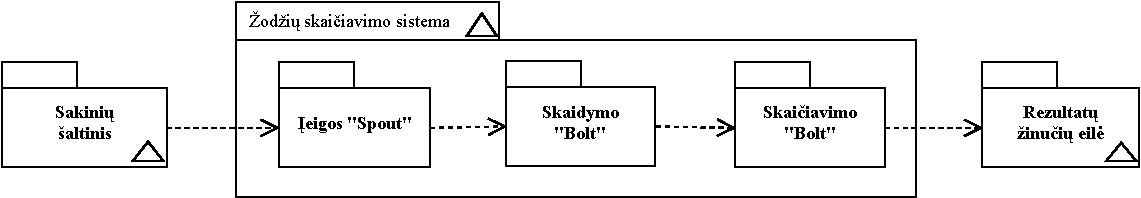
\includegraphics[width=1\textwidth]{img/pavyzdine_sistema.pdf}
    \caption{Srautinio apdorojimo sistemos pavyzdys}
    \label{img:example}
\end{figure}

\subsection{Pagal rodiklių duomenų modelį sugeneruotos srautinio apdorojimo sistemos}
Srautinio apdorojimo sistemos pagal rodiklių duomenų modelį generuojamos taip:
\begin{enumerate}
    \item Sugeneruojamas "Spout" tipo komponentas į kurį duomenys ateina iš žinučių eilės. Šis komponentas filtruoja duomenis pagal rodiklių duomenų modelyje apibrėžtus apribojimus. Taip pat šiame komponente prie pradinių rodiklių duomenų pridedama papildoma informacija: 
    \begin{itemize}
        \item Pirminis raktas sudarytas pagal rodiklių duomenų apibrėžimą ir pirminius rodiklių duomenis.
        \item Sugeneruotas unikalus identifikatorius, kuris naudojamas išvestinių rodiklių kombinacijos veiksmams.
    \end{itemize}
    \item Sugeneruojami "Bolt" tipo komponentai, pagal rodiklių duomenų modelio rodiklius. Pagal kiekvieną rodiklį sugeneruojamas vienas "Bolt" tipo komponentas.
    "Bolt" komponentai generuojami iš dviejų tipų rodiklių:
    \begin{itemize}
        \item Paprasti rodiklių "Bolt" komponentai, kurie iš pirminių duomenų ištraukia elementą, pagal raktą aprašyta rodiklio modelyje ir perduoda jį toliau.
        \item Išvestiniai rodiklių "Bolt" komponentai, kurie gauna duomenis iš vieno arba daugiau "Bolt" komponentų ir su jais atlieką transformacijos aprašytus rodiklio modelyje. Transformacijos gali būti bet kokie iš anksto aprašyti veiksmai su bet kokiu kiekiu duomenų. Pavyzdžiui: norint gauti išvestinį rodiklį, kuris skaičiuoja dviejų įeinančių rodiklių sumą turi būti:
        \begin{itemize}
            \item Srautinio apdorojimo sistemoje iš anksto aprašyta funkcija "suma", kuri priima du skaičius ir gražina vieną.
            \item Rodiklio modelyje transformacija aprašyta - suma(rodiklis1, rodiklis2).
        \end{itemize} 
    \end{itemize}
    \item Sugeneruojamas "Topology" aprašas, kuriame aprašomos "Spout" ir "Bolt" komponentų jungimaisi tarpusavyje pagal tai kaip jie aprašyti rodiklių duomenų modelyje. Visi paprastų rodiklių "Bolt" komponentai gauna duomenis iš "Spout", o išvestinių rodiklių "Bolt" komponentai gauna duomenis iš kitų paprastų arba išvestinių "Bolt" komponentų.
\end{enumerate}
Pavyzdžiui, jei turime rodiklį:     
\[
    \begin{tikzpicture}[sibling distance=10em,
        level distance=2cm,
        every node/.style = {shape=rectangle, rounded corners,	
                             draw, align=center,	
                             top color=white, bottom color=white}]	
        \node{Žmonių kaita\\Nuolatinė kaita + (Migracija * Gyventojų kiekis)}
                child { node {Nuolatinė kaita\\Gimstamumas - Mirtingumas} 
                        child {node {Mirtingumas}}
                        child {node {Gimstamumas}} }	
                child { node {Migracija} } 	
                child { node {Gyventojų kiekis} }; 	
    \end{tikzpicture} 	
\]
Tada sugeneruota srautinio apdorojimo sistema atrodys taip:
\begin{figure}[H]
    \centering
    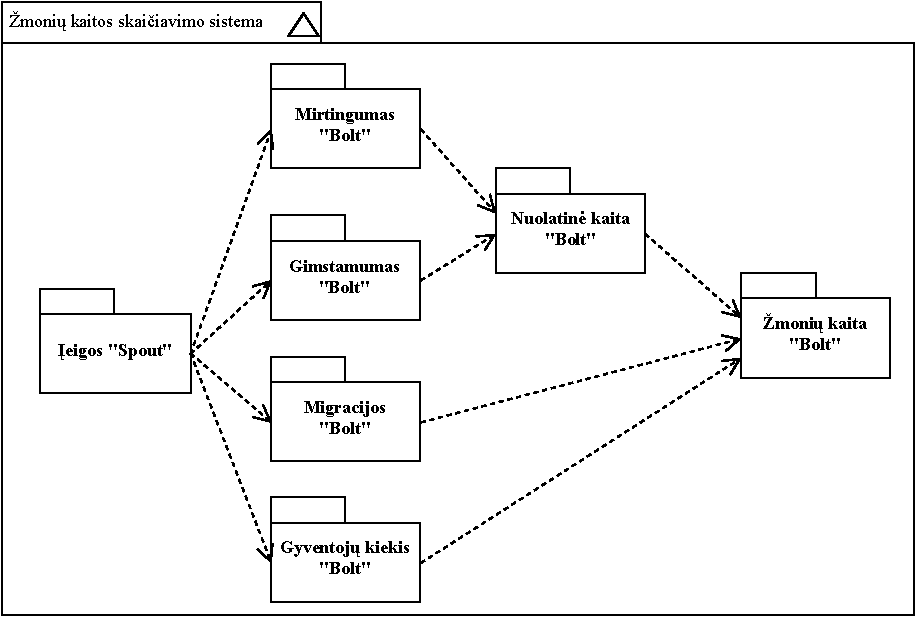
\includegraphics[width=1\textwidth]{img/generuota_sistema.pdf}
    \caption{Sugeneruotos srautinio apdorojimo sistemos pavyzdys}
    \label{img:example}
\end{figure}

\section{Eksperimentas ir sukurto sprendimo savybės}

\subsection{Eksperimento tikslas}

Nustatyti sukurto sprendimo ir architektūros savybes ir trukumus atliekant bandymus su rodiklių duomenimis:
\begin{enumerate}
    \item Sukurti sistemą apdorojančia rodiklius iš duomenų su apribojimais,.
    \item Esamai sistemai pridėti arba pašalinti apribojimą.
    \item Esamai sistemai pridėti rodiklį.
    \item Esamai sistemai pašalinti rodiklį. 
    \item Paduoti nereikalingus arba netinkamus duomenis į sistemą.
    \item Paduoti didelį kiekį duomenų vienu metu.
    \item Gauti apdorotus rodiklius.
    \item Gauti apdorotus rodiklius didelio duomenų kiekio padavimo į sistemą metu.
\end{enumerate}

\subsection{Eksperimento vykdymo aplinka}

Kompiuterio, kuriame buvo vykdomas eksperimentas specifikacijos:
\begin{itemize}
    \item Procesorius - Intel Core i7-7700k 4,5GHz
    \item Sisteminis diskas -  512 GB SSD
    \item Operatyvioji atmintis - 16 GB 
    \item Operacinė sistema - Ubuntu 18.04
\end{itemize}

\subsection{Kodo generavimo išpildymas}

Kodo generavimo komponentas - programinė įranga sukurta su .NET core biblioteka. Pasirinkta .NET core biblioteka, nes reikalingas "Web API" tašką (angl. endpoint) rodiklio modelis pateikimui. 
Kodo generavimas yra vykdomas pagal šablonus, kurie sukurti kiekvienam srautinio apdorojimo sprendimo komponento tipui. Šablono laukai, kuriuos reikia pakeisti, užrašyti specialiais identifikuojančiais elementais. Generavimo metu šie elementai keičiami reikiamu kodu užduočiai spręsti.
Šio komponento veikimas toks (\ref{img:generation-flow} pav.):
\begin{itemize}
    \item Taškas (angl. endpoint) rodiklių duomenų modelio pateikimui. Kadangi naudojama ".NET core" biblioteka buvo sukurtas "Web API" tipo projektas kuris leidžia kurti programinė įranga pagal REST architektūrą apibrėžtais taškais. Duomenis į tašką gali būti paduodami internetu, tai duoda privalumą - pats sprendimas gali būti kitame kompiuteryje arb kitame tinkle. Taip pat leidžia daug vartotojų dirbti su suskurtu sprendimu.
    \item Srautinio apdorojimo sistemų generavimas pagal pateiktą rodiklių duomenų modelį. Naudojant ".Net core" biblioteka generuojame Python kodą, kuris vėliau bus sukompiliuotas ir pateiktas srautinio apdorojo sprendimui. Kodo generavimas pradedamas tik gavus rodiklių duomenų modelį iš vartotojo. Eiga tokia:
    \begin{enumerate}
        \item Gaunamas rodiklių duomenų modelis.
        \item Patikriname ar egzistuoja tokia srautinio apdorojimo sistema. Tai darome kreipdamiesi į duomenų bazę ir tikrindami, ar egzistuoja įrašų, kurių rakto pradžia sutampa su generuojamos sistemos pavadinimu.
        \item Jei egzistuoja:
            \begin{enumerate}
                \item Sustabdome veikiančią sistemą. Tai darome kviesdami stabdymo komandą per Ubuntu operacinės terminalą.
                \item Iš duomenų bazės traukiame jau apdorotus rodiklių duomenis ir juos perduodame į generavimo dalį.
            \end{enumerate} 
        \item Generuojame srautinio apdorojimo sistemos įeigos komponentą - įrašome žinučių eilės grupės pavadinimą, parašome sąlygas įeinantiems duomenims pagal apribojimus ir sugeneruojame unikalų identifikatorių duomeniui, kurio pagalba toliau einantys veiksmai, kurie reikalauja duomenų apdorojimo iš kelių skirtingų komponentų, sukombinuoja duomenis.
        \item Pagal rodiklius rekursyviai generuojame duomenų apdorojimo komponentus, jei tai jau egzistuojantis komponentas užpildome jį apdorotais duomenimis gautais iš duomenų bazės. 
        \item Generuojama sistemos topologiją, kuri aprašo komponentų jungimosi tarpusavyje logiką, komponentų paralelizmo lygi ir kitas sistemos konfigūracijas. 
        \item Visos sugeneruotos bylos talpinamos į vieną aplanką ir paleidžiamas specialus įrankis kompiliavimui.
        \item Sukompiliuota sistema pateikiama į srautinio apdorojimo programą.
    \end{enumerate}
    \item Srautinio apdorojimo sistemų teikimo ir trynimo operacijos su srautinio apdorojimo sprendimu.
    \item Apdorotų rodiklių traukimas iš duomenų bazės ir naudojimas perkuriant jau egzistuojančią srautinio apdorojimo sistemą.
\end{itemize}

\begin{figure}[H]
    \centering
    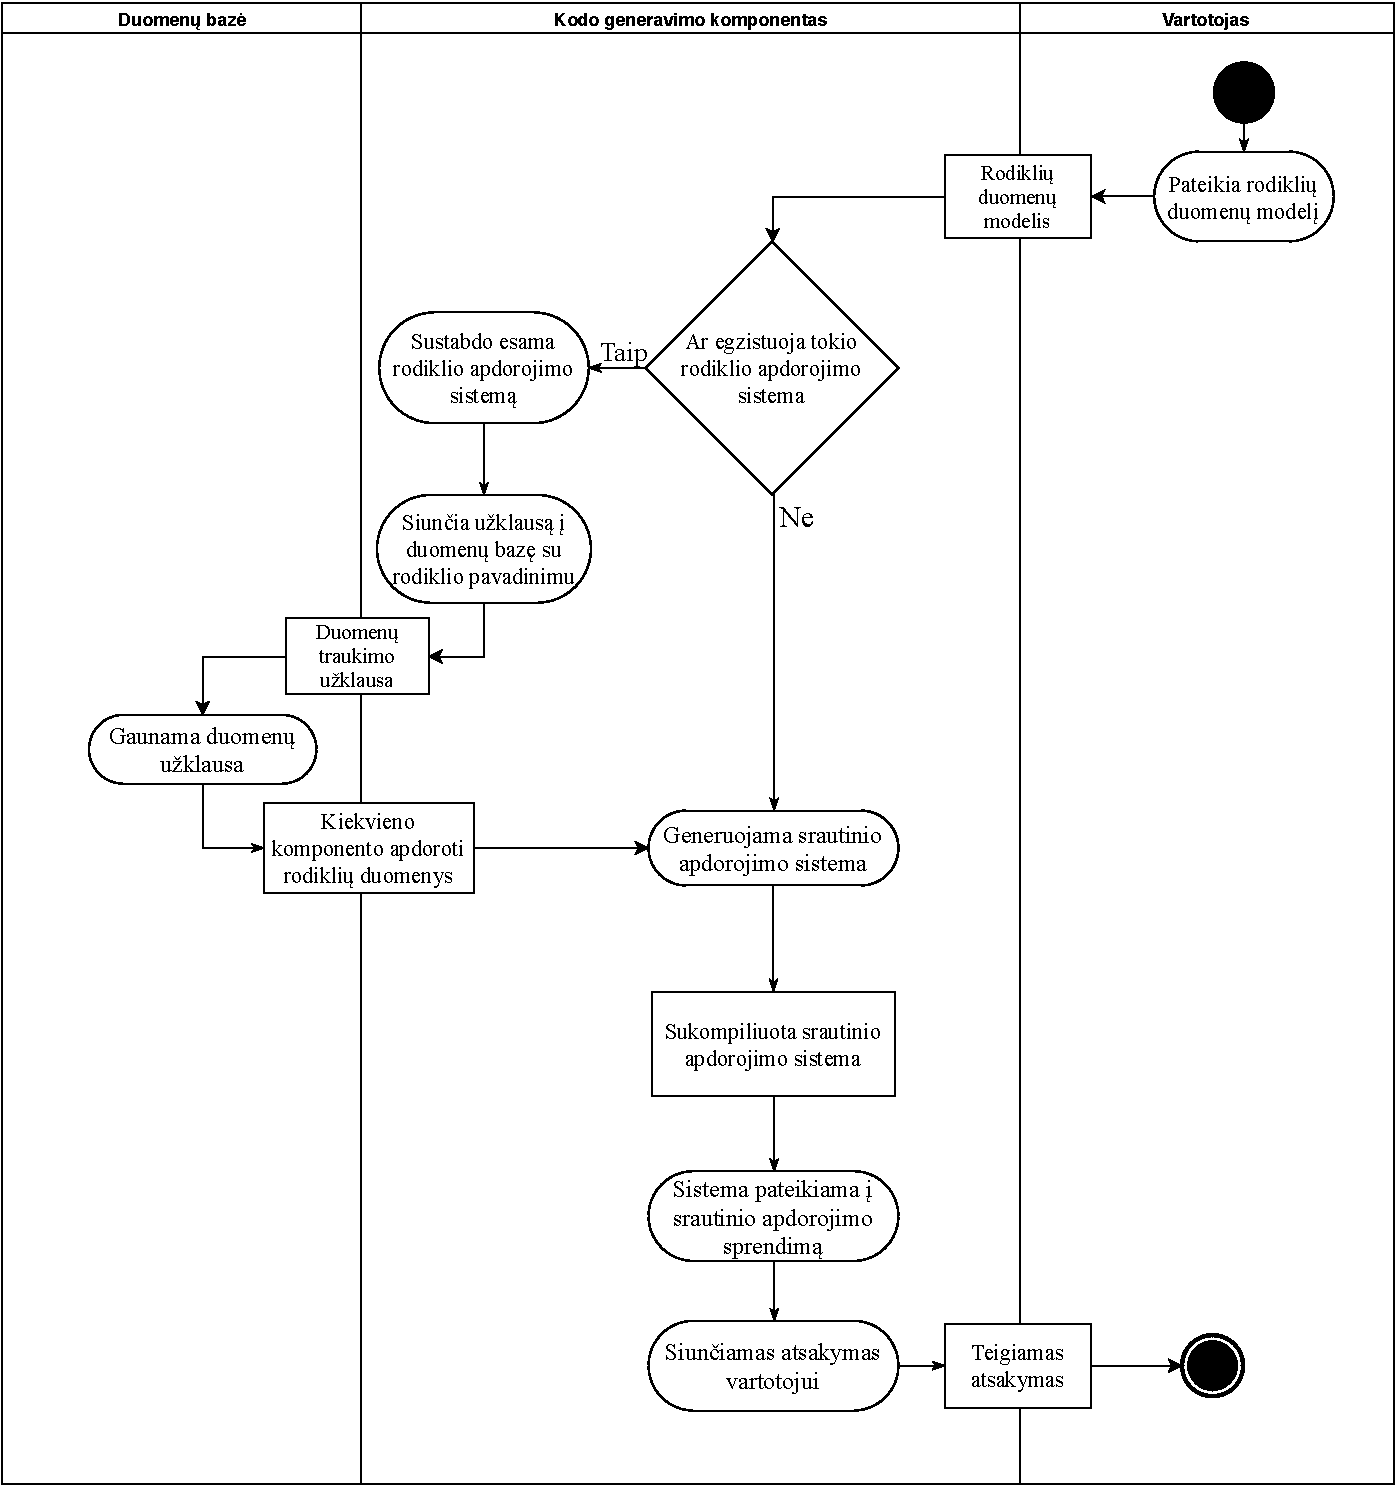
\includegraphics[width=1\textwidth]{img/generation-flow.pdf}
    \caption{Kodo generavimo komponento veikimas}
    \label{img:generation-flow}
\end{figure}

\subsection{Apdorotų rodiklių duomenų bazė}

Duomenų bazė koncepciniam sprendime saugos apdorotus rodiklių duomenis. Duomenys šioje duomenų bazėje bus tik įrašomi ir skaitomi. Kadangi mes norime turėti apdorotus išvestinių ir pagrindinių rodiklių duomenis, visi srautinio apdorojimo sistemų komponentai turės prisijungti prie duomenų bazės ir padėti paskutinę apdorotų duomenų versiją. Duomenys iš duomenų bazės bus traukiami dviem poreikiam: 
\begin{enumerate}
    \item Vartotojui norint gauti apdorotus rodiklių duomenis, vartotojas sius užklaus į architektūroje padarytą prieigos tašką pateikdamas rodiklio pavadinimą ir gaus atsakymą su jau apdorotais rodikliais. 
    \item Kodo generavimo komponentas naudos apdorotų rodiklių duomenis, kai bus pergeneruojamos srautinio apdorojimo sistemos.  Kadangi po rodiklių pridėjimo arba pašalinimo mes norime, kad nepakeistų rodiklių apdorojimas vyktų toliau, po srautinio apdorojimo sistemos sustabdymo, kodo generavimo komponentas trauks paskutinius apdorojamus duomenis ir dės juos į jau esamus srautinio apdorojimo sistemos komponentus. Taip bus užtikrinamas duomenų apdorojimo pratesimas.   
\end{enumerate}  

Saugoti apdorotus duomenis buvo pasirinkta "Redis" duomenų bazę. Ji pasirinkta kadangi apdoroti rodiklių duomenis užima nedaug vietos ir svarbu greitai pasiekti ir įdėti duomenis. "Redis" duomenų bazių valdymo sistema tinka, nes duomenis saugomi operatyvioj atmintyje. Apdoroti rodikliai saugomi unikalioje eilėje pagal rodiklio modelio ir apdorojamo rodiklio pavadinimo kombinacija. Pavyzdžiui: renkant darbuotojų atlyginimus per metus iš uždarbio ir premijos, apdoroti rodiklių duomenys būtų saugomi pagal raktus: "darbuotojų-atlyginimas:uždarbis", "darbuotojų-atlyginimas:premijos" ir "darbuotojų-atlyginimas:atlyginimas"


\subsection{Papildoma programinė įranga}

Pilnam sistemos veikimui taip pat reikia papildomos programinės įrangos, kurį užsiima duomenų perdavimu, srautinio apdorojimo sistemų kompiliavimu. Ši įranga naudojama tokia kaip pateikiama nekeičiant konfigūracijos iš esmės.
\begin{itemize}
    \item Žinučių eilės pagrindinis uždavinys - perduoti duomenis į srautinio apdorojimo sistemą. Žinučių eilės naudoja publikavimo-prenumeratos modelį (angl. publish-subscribe pattern), komponentai norintys gauti duomenis užsiregistruoja žinučių eilėje, o komponentai siunčiantis tiesiog perduoda juos į žinučių eilę. Taip yra įgyvendinamas asinchroninis bendravimas, komponentai perduoda duomenis į žinučių eilę, o komponentas norintis gauti duomenis gali juos pasiimti bet kuriuo momentu iš eilės. Koncepcinio sprendimo įgyvendinimui pasirinkta Apache Kafka žinučių eilė.
    \item Apache Kafka reikalauja Apache Zookeeper, kuris atsakingas už Apache Kafka žinučių eilės konfigūracijos valdymą.
    \item Sugeneruotos sistemos kompiliavimui naudojama "Pants" kompiliavimo sistema.
\end{itemize}

Testavimo duomenų generatorius, Postman, naršyklė

\subsection{Eksperimento eiga}

\subsection{Eksperimento išvados}

\subsection{Sprendimo savybės}

\sectionnonum{Rezultatai}

\begin{enumerate}
    \item Apibrėžta rodiklių duomenų struktūra ir galimi duomenų struktūros pokyčiai.
    \item Sukurtas architektūra tinkama spręsti rodiklių apdorojimo uždavinį. 
    \item Pasirinktam srautinio apdorojimo sprendimui, pagal sukurtą architektūra sukurtas sprendimas
    \item Atlikti eksperimentai su sukurtu sprendimu ir apžvelgtos jo savybės. 
\end{enumerate}

\sectionnonum{Išvados}
\begin{itemize}
    \item Išvada 1
    \item Išvada 2 
\end{itemize}

\printbibliography[heading=bibintoc] 


% \appendix 


\end{document}
